\documentclass{standalone}
\usepackage{tikz}
\usetikzlibrary{patterns, positioning}


\begin{document}
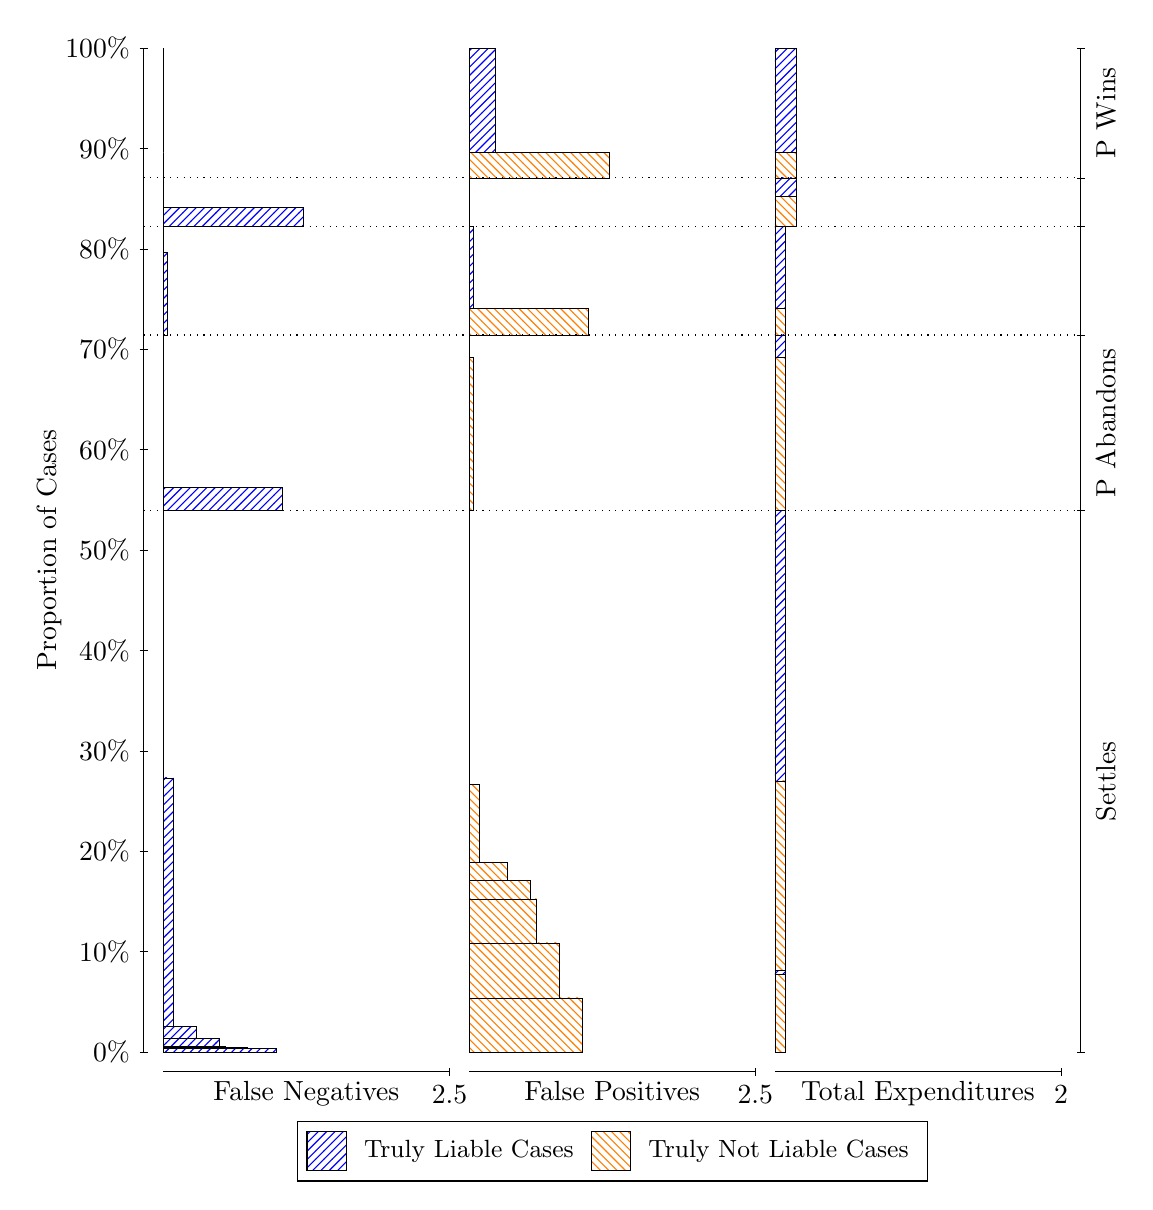
\begin{tikzpicture}
\draw[black, very thin] (1.5,1.75) -- (1.5,14.5);
\node[rotate=90, text=black, anchor=center] at (0.3, 8.125) {Proportion of Cases};
\draw[black, very thin] (1.45,1.75) -- (1.55,1.75);
\node[text=black, anchor=east] at (1.45, 1.75) {0\%};
\draw[black, very thin] (1.45,3.025) -- (1.55,3.025);
\node[text=black, anchor=east] at (1.45, 3.025) {10\%};
\draw[black, very thin] (1.45,4.3) -- (1.55,4.3);
\node[text=black, anchor=east] at (1.45, 4.3) {20\%};
\draw[black, very thin] (1.45,5.575) -- (1.55,5.575);
\node[text=black, anchor=east] at (1.45, 5.575) {30\%};
\draw[black, very thin] (1.45,6.85) -- (1.55,6.85);
\node[text=black, anchor=east] at (1.45, 6.85) {40\%};
\draw[black, very thin] (1.45,8.125) -- (1.55,8.125);
\node[text=black, anchor=east] at (1.45, 8.125) {50\%};
\draw[black, very thin] (1.45,9.4) -- (1.55,9.4);
\node[text=black, anchor=east] at (1.45, 9.4) {60\%};
\draw[black, very thin] (1.45,10.675) -- (1.55,10.675);
\node[text=black, anchor=east] at (1.45, 10.675) {70\%};
\draw[black, very thin] (1.45,11.95) -- (1.55,11.95);
\node[text=black, anchor=east] at (1.45, 11.95) {80\%};
\draw[black, very thin] (1.45,13.225) -- (1.55,13.225);
\node[text=black, anchor=east] at (1.45, 13.225) {90\%};
\draw[black, very thin] (1.45,14.5) -- (1.55,14.5);
\node[text=black, anchor=east] at (1.45, 14.5) {100\%};

\draw[black, very thin] (13.4,1.75) -- (13.4,14.5);
\draw[black, very thin] (13.35,1.75) -- (13.45,1.75);
\node[anchor=west] at (13.35, 1.75) {};
\draw[black, very thin] (13.35,8.6287) -- (13.45,8.6287);
\node[anchor=west] at (13.35, 8.6287) {};
\draw[black, very thin] (13.35,10.856) -- (13.45,10.856);
\node[anchor=west] at (13.35, 10.856) {};
\draw[black, very thin] (13.35,12.238) -- (13.45,12.238);
\node[anchor=west] at (13.35, 12.238) {};
\draw[black, very thin] (13.35,12.851) -- (13.45,12.851);
\node[anchor=west] at (13.35, 12.851) {};
\draw[black, very thin] (13.35,14.5) -- (13.45,14.5);
\node[anchor=west] at (13.35, 14.5) {};

\draw[black, very thin, pattern color=blue, pattern=north east lines] (1.75,1.75) rectangle (3.1852,1.7946);
\draw[black, very thin, pattern color=blue, pattern=north east lines] (1.75,1.7946) rectangle (2.8218,1.8061);
\draw[black, very thin, pattern color=blue, pattern=north east lines] (1.75,1.8061) rectangle (2.5312,1.8188);
\draw[black, very thin, pattern color=blue, pattern=north east lines] (1.75,1.8188) rectangle (2.4585,1.9215);
\draw[black, very thin, pattern color=blue, pattern=north east lines] (1.75,1.9215) rectangle (2.1678,2.0761);
\draw[black, very thin, pattern color=blue, pattern=north east lines] (1.75,2.0761) rectangle (1.8772,5.2305);
\draw[black, very thin, pattern color=orange, pattern=north west lines] (1.75,5.2305) rectangle (1.75,8.6287);
\draw[black, very thin, pattern color=blue, pattern=north east lines] (1.75,8.6287) rectangle (3.2578,8.9176);
\draw[black, very thin, pattern color=orange, pattern=north west lines] (1.75,8.9176) rectangle (1.75,10.856);
\draw[black, very thin, pattern color=blue, pattern=north east lines] (1.75,10.856) rectangle (1.8045,11.904);
\draw[black, very thin, pattern color=orange, pattern=north west lines] (1.75,11.904) rectangle (1.75,12.238);
\draw[black, very thin, pattern color=blue, pattern=north east lines] (1.75,12.238) rectangle (3.5303,12.472);
\draw[black, very thin, pattern color=orange, pattern=north west lines] (1.75,12.472) rectangle (1.75,12.851);
\draw[black, very thin, pattern color=orange, pattern=north west lines] (1.75,12.851) rectangle (1.75,13.176);
\draw[black, very thin, pattern color=blue, pattern=north east lines] (1.75,13.176) rectangle (1.75,14.5);
\draw[black, very thin, pattern color=orange, pattern=north west lines] (5.6333,1.75) rectangle (7.0685,2.436);
\draw[black, very thin, pattern color=orange, pattern=north west lines] (5.6333,2.436) rectangle (6.7778,3.135);
\draw[black, very thin, pattern color=orange, pattern=north west lines] (5.6333,3.135) rectangle (6.4872,3.6951);
\draw[black, very thin, pattern color=orange, pattern=north west lines] (5.6333,3.6951) rectangle (6.4145,3.9287);
\draw[black, very thin, pattern color=orange, pattern=north west lines] (5.6333,3.9287) rectangle (6.1238,4.1593);
\draw[black, very thin, pattern color=orange, pattern=north west lines] (5.6333,4.1593) rectangle (5.7605,5.1483);
\draw[black, very thin, pattern color=blue, pattern=north east lines] (5.6333,5.1483) rectangle (5.6333,8.6287);
\draw[black, very thin, pattern color=orange, pattern=north west lines] (5.6333,8.6287) rectangle (5.6878,10.568);
\draw[black, very thin, pattern color=blue, pattern=north east lines] (5.6333,10.568) rectangle (5.6333,10.856);
\draw[black, very thin, pattern color=orange, pattern=north west lines] (5.6333,10.856) rectangle (7.1412,11.19);
\draw[black, very thin, pattern color=blue, pattern=north east lines] (5.6333,11.19) rectangle (5.6878,12.238);
\draw[black, very thin, pattern color=orange, pattern=north west lines] (5.6333,12.238) rectangle (5.6333,12.618);
\draw[black, very thin, pattern color=blue, pattern=north east lines] (5.6333,12.618) rectangle (5.6333,12.851);
\draw[black, very thin, pattern color=orange, pattern=north west lines] (5.6333,12.851) rectangle (7.4137,13.176);
\draw[black, very thin, pattern color=blue, pattern=north east lines] (5.6333,13.176) rectangle (5.9603,14.5);
\draw[black, very thin, pattern color=orange, pattern=north west lines] (9.5167,1.75) rectangle (9.6529,2.739);
\draw[black, very thin, pattern color=blue, pattern=north east lines] (9.5167,2.739) rectangle (9.6529,2.7836);
\draw[black, very thin, pattern color=orange, pattern=north west lines] (9.5167,2.7836) rectangle (9.6529,5.1929);
\draw[black, very thin, pattern color=blue, pattern=north east lines] (9.5167,5.1929) rectangle (9.6529,8.6287);
\draw[black, very thin, pattern color=orange, pattern=north west lines] (9.5167,8.6287) rectangle (9.6529,10.568);
\draw[black, very thin, pattern color=blue, pattern=north east lines] (9.5167,10.568) rectangle (9.6529,10.856);
\draw[black, very thin, pattern color=orange, pattern=north west lines] (9.5167,10.856) rectangle (9.6529,11.19);
\draw[black, very thin, pattern color=blue, pattern=north east lines] (9.5167,11.19) rectangle (9.6529,12.238);
\draw[black, very thin, pattern color=orange, pattern=north west lines] (9.5167,12.238) rectangle (9.7892,12.618);
\draw[black, very thin, pattern color=blue, pattern=north east lines] (9.5167,12.618) rectangle (9.7892,12.851);
\draw[black, very thin, pattern color=orange, pattern=north west lines] (9.5167,12.851) rectangle (9.7892,13.176);
\draw[black, very thin, pattern color=blue, pattern=north east lines] (9.5167,13.176) rectangle (9.7892,14.5);
\draw[black, dotted] (1.5,8.6287) -- (13.4,8.6287);
\draw[black, dotted] (1.5,10.856) -- (13.4,10.856);
\draw[black, dotted] (1.5,12.238) -- (13.4,12.238);
\draw[black, dotted] (1.5,12.851) -- (13.4,12.851);
\draw[black, very thin] (1.75,1.5) -- (5.3833,1.5);
\node[text=black, anchor=north] at (3.5667, 1.5) {False Negatives};
\draw[black, very thin] (5.3833,1.45) -- (5.3833,1.55);
\node[text=black, anchor=north] at (5.3833, 1.45) {2.5};

\draw[black, very thin] (5.6333,1.5) -- (9.2667,1.5);
\node[text=black, anchor=north] at (7.45, 1.5) {False Positives};
\draw[black, very thin] (9.2667,1.45) -- (9.2667,1.55);
\node[text=black, anchor=north] at (9.2667, 1.45) {2.5};

\draw[black, very thin] (9.5167,1.5) -- (13.15,1.5);
\node[text=black, anchor=north] at (11.333, 1.5) {Total Expenditures};
\draw[black, very thin] (13.15,1.45) -- (13.15,1.55);
\node[text=black, anchor=north] at (13.15, 1.45) {2};

\node[text=black, centered, rotate=90] at (13.72, 5.1894) {Settles};
\node[text=black, centered, rotate=90] at (13.72, 9.7426) {P Abandons};


\node[text=black, centered, rotate=90] at (13.72, 13.676) {P Wins};

\draw (7.449999999999999,1.5) node[draw=none] (baseCoordinate) {};
\begin{scope}[align=center]
        \matrix[scale=0.5, draw=black, below=0.5cm of baseCoordinate, nodes={draw}, column sep=0.1cm]{
            \node[rectangle, draw, minimum width=0.5cm, minimum height=0.5cm, pattern color=blue, pattern=north east lines] {}; &
            \node[draw=none, font=\small, text=black] (B) {Truly Liable Cases}; &
            \node[rectangle, draw, minimum width=0.5cm, minimum height=0.5cm, pattern color=orange, pattern=north west lines] {}; &
            \node[draw=none, font=\small, text=black] (B) {Truly Not Liable Cases}; \\
            };
\end{scope}

\end{tikzpicture}
\end{document}